\section{{\bf PLAN}}
What will we do...





\subsection{ASTR 490} 

Was it 490? Andy remembers...


Copied text from that email, which was copied from our book, to see
how many pages it would take...

\subsubsection{Motivation for Astr 490}

Astronomy and astrophysics are witnessing dramatic increases in data volume 
as detectors, telescopes, and computers become ever more powerful. During the 
last decade, sky surveys across the electromagnetic spectrum have collected 
hundreds of terabytes of astronomical data for hundreds of millions of sources. 
Over the next decade, the data volume will enter the petabyte domain, and provide 
accurate measurements for billions of sources. Astronomy and physics students 
are not traditionally trained to handle such voluminous and complex data sets. 
Furthermore, standard analysis methods employed in astronomy often lag far 
behind rapid progress in statistics and computer science. The main
goal of this course is to contribute to efficient training of next
generations of students to 
handle the fast growing data sets, not only in astronomy, but in other quantitative 
sciences as well. 

This course will be aimed at physical and data-centric math,
statistics, science and engineering students
who have an understanding of the science drivers for analyzing large data sets but 
may not be aware of appropriate statistical techniques for doing so. The course work 
will provide to students a connection between scientific data analysis problems and 
modern statistical methods. We will limit theoretical discussions to the minimum 
required to understand the algorithms and will build the courses upon an 
example-driven compendium of modern statistical and data mining methods, 
together with carefully chosen examples based on real modern data sets, and of 
current astronomical applications that will illustrate each method introduced in the 
book. Discussion of the advanced material will be supported by appropriate (publicly 
available) Python code and data which will enable students to perform exercises, 
evaluate the techniques, and adapt them to their own fields of interest. We chose to 
use Python, a powerful and flexible programming language that is quickly becoming 
a standard in data-intensive sciences (and elsewhere). 

The target audience for our course includes undergraduate students with scientific 
or engineering background, but it is likely that graduate students
would benefit from it too. Familiarity with calculus and other basic mathematical 
techniques will be assumed, but no extensive prior knowledge in statistics will be 
required. 

The course outline: 

\begin{enumerate} 
\item Computational Challenges in data-intensive astronomy and astrophysics
\begin{itemize}
\item  data types and data management systems 
\item  analysis of algorithmic efficiency
\item  types of computational problems and strategies for speeding them up 
\item  data visualization challenges
\item  selection effects and truncated/censored data in astronomical context 
\end{itemize}
\item Searching for structure in astronomical point data
\begin{itemize}
\item  non-parametric density estimation
\item  nearest-neighbor density estimation
\item  parametric density estimation
\item  finding clusters in data 
\item  correlation functions 
\end{itemize} 
\item Dimensionality reduction
\begin{itemize}
\item  principal component analysis in astronomical context
\item  non-negative matrix factorization 
\item  independent component analysis and projection pursuit 
\item  manifold learning
\end{itemize} 
\item Regression and model fitting
\begin{itemize}
\item  regresion for linear models
\item  non-linear regression
\item  kernel and principal component regression
\item  methods for handling heteroscedastic and non-Gaussian errors 
\item  Gaussian processes
\item  overfitting, underfitting and cross-validation
\end{itemize} 
\item Classification 
\begin{itemize}
\item  generative classification methods
\item  discriminative classification method 
\item  evaluation and comparison of classifiers: ROCcurves 
\end{itemize} 
\item Time series analysis in astronomy
\begin{itemize}
\item  main concepts and tools for time series analysis
\item  analysis of periodic time series 
\item  temporally localized signals
\item  analysis of stochastic processes
\end{itemize} 
\end{enumerate} 


We will textbook {\it ``Statistics, Data Mining, and Machine Learning in Astronomy:
A Practical Python Guide for the Analysis of Survey Data''} (Princeton Series in Modern 
Observational Astronomy) coauthored by Co-PIs on this prooposal. 


\subsection{Python Packages} 



We will leverage all the publicly available modern python tools. 
In particular,  seminar work will be built around the {\it astroML} package
that was developed to support textbook to be used with the proposed course. 


\begin{figure*}[!t]
\vskip -5.5in
\includegraphics[width=1.02\hsize,clip]{astroML.eps}
\vskip -2.0in
\caption{We will leverage all the modern python tools available in {\it astroML} and
other packages.} 
\label{Fig:astroML}
\end{figure*}




\subsection{Workshop} 


At the last meeting, we assumed a 3-day workshop for about 30 faculty from other institutions
of higher learning who would want to emulate our program. Further assuming \$20/day/person
for lunch and coffee, and \$75/person for conference dinner, \$1,500 for the workshop venue,
and four grants of \$500 to young faculty and postdocs, we need about \$7,500 for the workshop. 



\subsection{Budget} 

We assumed a 3-year long project. 

We assumed 2.5 months of summer salary for Marina, and a postdoc. About \$150,000/year. 

We assumed 1 month of summer salary for both \v{Z}I and Andy to demonstrate seriousness,
and a graduate student. About \$100,000/year. 

All together, about \$750,000 for 3 years. If this is above the limit, perhaps we could 
descope faculty to only the first two years? 



